\documentclass[
	%sans,			% use sans-serif font
	%serif,			% use serif-font
	%mathsans,		% set mathtext to sans-serif
	%mathserif,		% set mathtext to serif
	%10pt,
	10pt,
	%12pt,
	t		% add text at the top border of slide
	%slidescentered,% center text on slide
	%draft,			% compile as draft version
	%handout,		% create handout file
	%notes,			% include nodes in slides
	%compress		% compress navigation bar
]{beamer}

\usetheme{lmtslides}
\usepackage{eso-pic}
\usepackage{graphicx}
%\usepackage[pdftex]{color}
\usepackage{times}
\usepackage[latin1]{inputenc}
%\usepackage[T1]{fontenc}
\usepackage[amssymb]{SIunits}
\usepackage{amsmath,amssymb}
\usepackage{eurosym}
\usepackage{booktabs}
\usepackage{colortbl}
\usepackage{url}
\usepackage[absolute,overlay]{textpos}
\usepackage{graphicx}
\usepackage{mathtools}

\renewcommand{\footnoterule}{\vfill\kern -3pt  \kern 2.6pt}

\setbeamertemplate{caption}{\raggedright\insertcaption\par}
\setbeamertemplate{bibliography item}[online]
\graphicspath{{figures/}}

\setlang{en}		

% Supervisor: Univ.-Prof. Dr. Hans-Joachim Bungartz
% Advisors: Manish Kumar Mishra, M.Sc. (hons) &
% Samuel James Newcome, M.Sc.

% MODIFY THESE ACCORDINGLY! ---
\title{Exploring Fuzzy Tuning Technique for Molecular Dynamics Simulations in AutoPas}
\type{Bf} % (M/B/D/S)(f/m): (Master/Bachelor/Diplom/Studienarbeit)(final/midterm)
\author{Manuel Lerchner}
\email{manuel.lerchner@tum.de}
\advisorOne{Manish Kumar Mishra, M.Sc. (hons)}
\advisorTwo{Samuel James Newcome, M.Sc.}
\date{\today}
%------------------------------


%%%%%%%%%%%%%%%%%%%%%%%%%%
\begin{document}

\maketitle
\thispagestyle{empty}

\begin{frame}[noframenumbering]
	\frametitle{Table of Contents}
	\tableofcontents
\end{frame}

\setcounter{framenumber}{0}


\section{What is AutoPas?}
\begin{frame}
	\frametitle{What is AutoPas?}

	\begin{textblock*}{5cm}(9cm,1.8cm)
		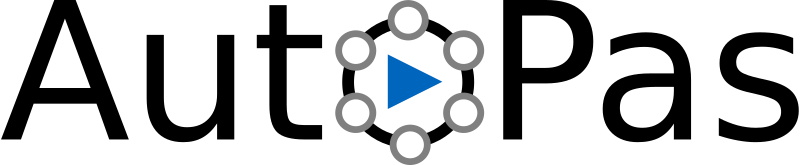
\includegraphics[width=3cm]{figures/AutoPasLogo}
	\end{textblock*}


	\begin{itemize}
		\item Library for optimal node-level performance in N-body simulations
		\item Many different implementations for the N-body problem
		\item AutoTuning: Automatically switch between implementations
		      \begin{itemize}
			      \item \textbf{Container:} How to find neighboring particles?
			      \item \textbf{Traversal:} How to efficiently handle multi-threading?
			      \item \textbf{Data Layout:} How to store particles in memory?
			      \item \textbf{Newton 3:} Can we exploit Newton's 3rd law?
			      \item \dots
		      \end{itemize}
		\item Example applications:
		      \begin{itemize}
			      \item \texttt{md\_flexible} (Molecular Dynamics)
			      \item \texttt{sph} (Smoothed Particle Hydrodynamics)
			      \item Space Debris Collision Modelling
		      \end{itemize}
	\end{itemize}
\end{frame}


\begin{frame}
	\frametitle{Structure of AutoPas}

	\begin{itemize}
		\item Three main areas:
		      \begin{itemize}
			      \item User Application
			      \item Algorithm Library
			      \item Tuning Strategies
		      \end{itemize}
		\item Algorithm Library:
		      \begin{itemize}
			      \item Huge Search Space\footnote{\scriptsize{$\text{Container}\times\text{Traversal} \times \text{Data Layout} \times \text{Newton 3} \times \text{Load Estimator} \times \text{Cell Size Factor}$}
			            }
		      \end{itemize}
		\item Tuning Strategies:
		      \begin{itemize}
			      \item Full Search
			      \item Random Search
			      \item Predictive Tuning
			      \item Bayesian Search
			      \item Rule Based Tuning
		      \end{itemize}
	\end{itemize}

	\begin{textblock*}{4cm}(8cm,2cm)
		\begin{figure}
			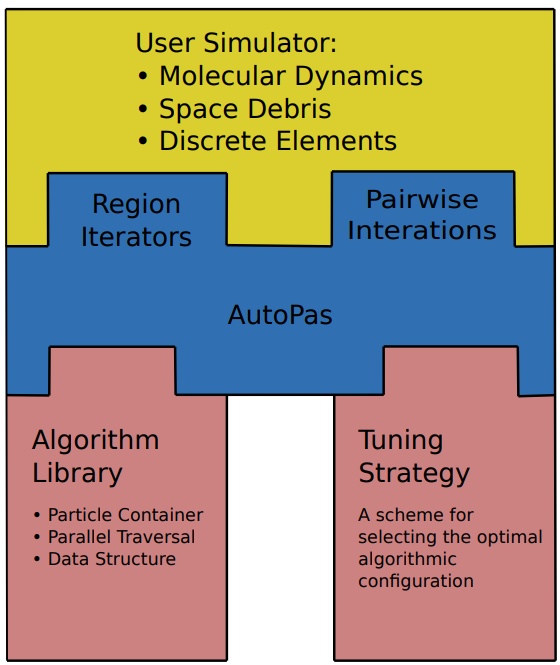
\includegraphics[width=4cm]{figures/AutoPasLibraryStructure.png}
			\caption{ \footnotesize{Source: \cite{Newcome2023Poster}}}

		\end{figure}
	\end{textblock*}
\end{frame}



\begin{frame}
	\frametitle{Auto-Tuning }

	\begin{itemize}
		\item Tuning Phase: Find the best configuration
		      \begin{itemize}
			      \item Tuning Strategies select promising configurations to evaluate
			      \item All those configurations are evaluated and measured
			      \item Huge overhead, if done badly
		      \end{itemize}
		\item Simulation Phase: Use the best configuration
	\end{itemize}

	\vspace{0.1cm}

	\begin{center}
		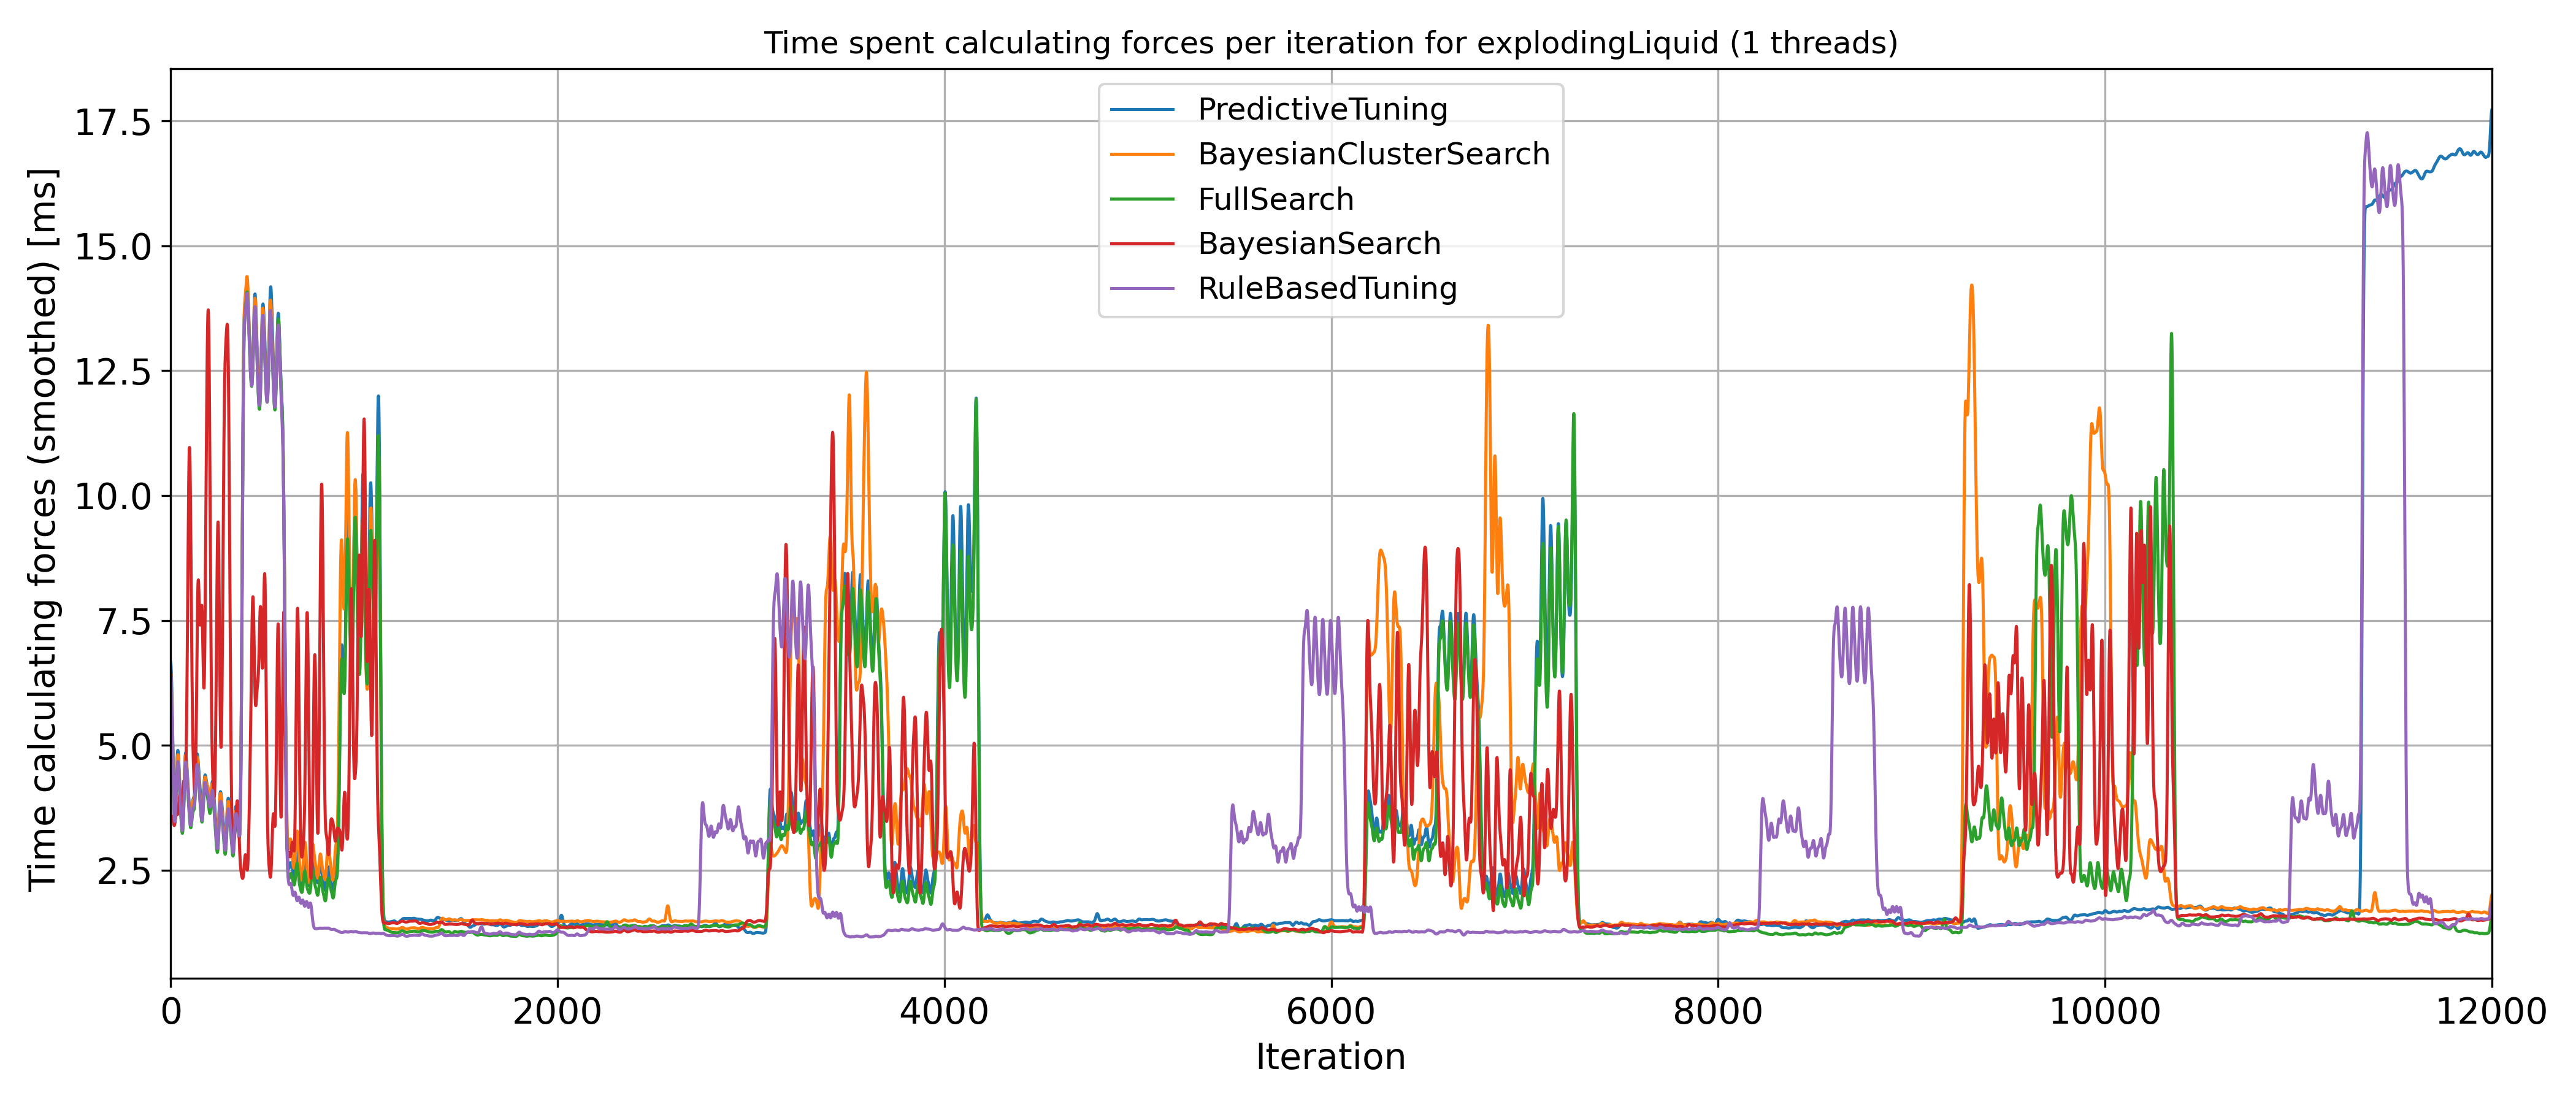
\includegraphics[width=0.95\textwidth,trim={0 0 0 0.85cm},clip]{figures/timing_explodingLiquid.png}
	\end{center}


\end{frame}

\section{Mathematics of Fuzzy Logic}
\begin{frame}
	\frametitle{Fuzzy Logic Systems}

	\begin{itemize}
		\item Use human-like reasoning to model complex systems
		\item Linguistic Terms (\textit{cold, hot, \dots}) reduce complexity in modeling
		      \begin{itemize}
			      \item Smooth transitions between terms (e.g. \textit{cold} $\rightarrow$ \textit{warm})
		      \end{itemize}
		\item Fuzzy Systems are functions $f: \mathbb{R}^n \rightarrow \mathbb{R}$
		\item Rule based: Easy to understand, interpret and adapt
		      \begin{itemize}
			      \item Interpolation effect between regions and conflicting rules
			      \item No hard boundaries $\rightarrow$ robust against noise
		      \end{itemize}
	\end{itemize}

	\begin{example}[Heater Control]

		\begin{description}[wide=0]
			\item[\textbf{Input:}  ] ~ temperature (e.g. 20$^{\circ}$C), humidity (e.g. 50\%)
			\item[\textbf{Output:}] heater power (e.g. 50\%)
			\item[\textbf{Rules:}]
			      {\footnotesize
			      \begin{tabular}{lcll}
				      \textbf{IF}  temp is \textit{cold} & \textbf{AND} & humidity is \textit{dry} & \textbf{THEN}  power is \textit{high}   \\
				      \textbf{IF}  temp is \textit{hot}  & \textbf{OR}  & humidity is \textit{wet} & \textbf{THEN}  power is \textit{low}    \\
				      \textbf{IF}  temp is \textit{warm} &              &                          & \textbf{THEN}  power is \textit{medium} \\
			      \end{tabular} }
		\end{description}
	\end{example}

\end{frame}

\begin{frame}
	\frametitle{Naming Conventions}

	\begin{itemize}
		\item Consider the Fuzzy Rule:
		      \[
			      \underbrace{  \underbrace{\textbf{IF}  \;\underbrace{\text{temp}}_{\text{Ling. Var.}} \text{is} \underbrace{\textit{cold}}_{\text{Ling. Term}}  \textbf{AND}  \underbrace{\text{hum}}_{\text{Ling. Var.}} \text{is} \underbrace{\textit{dry}}_{\text{Ling. Term}} }_{\text{Antecedent}}
				      \textbf{THEN}  \underbrace{\underbrace{\text{power}}_{\text{Ling. Var.}} \text{is} \underbrace{\textit{high}}_{\text{Ling. Term}}}_{\text{Consequent}}
			      }_{\text{Fuzzy Rule}}
		      \]
		\item Fuzzy Logic Systems consist of:
		      \begin{itemize}
			      \item Linguistic Terms / Fuzzy Sets (e.g. \textit{cold, warm, hot})
			      \item Linguistic Variables (e.g. temperature, humidity, power)
			      \item Fuzzy Logic Operators (e.g. \textbf{AND, OR, NOT})
			      \item Fuzzy Rules (e.g. \textbf{IF} \textit{antecedent} \textbf{THEN} \textit{consequent})
		      \end{itemize}
	\end{itemize}
\end{frame}

\begin{frame}
	\frametitle{Fuzzy Sets vs Classical Sets}
	\begin{itemize}
		\item Fuzzy Sets are generalizations of classical sets
		      \begin{itemize}
			      \item $U$ is the universe of discourse (e.g. $age \subseteq \mathbb{R}$)
			      \item Classical Set $A \subseteq U$:
			            \begin{itemize}
				            \item Defined via indicator function $\chi_A : U \rightarrow \{0,1\}$
			            \end{itemize}
			      \item Fuzzy Sets $\tilde{A} \subseteq U$:
			            \begin{itemize}
				            \item Defined via \textbf{Continuous} membership function $\mu_{\tilde{A}} : U  \rightarrow [0,1]$
			            \end{itemize}
		      \end{itemize}
	\end{itemize}
	\begin{center}
		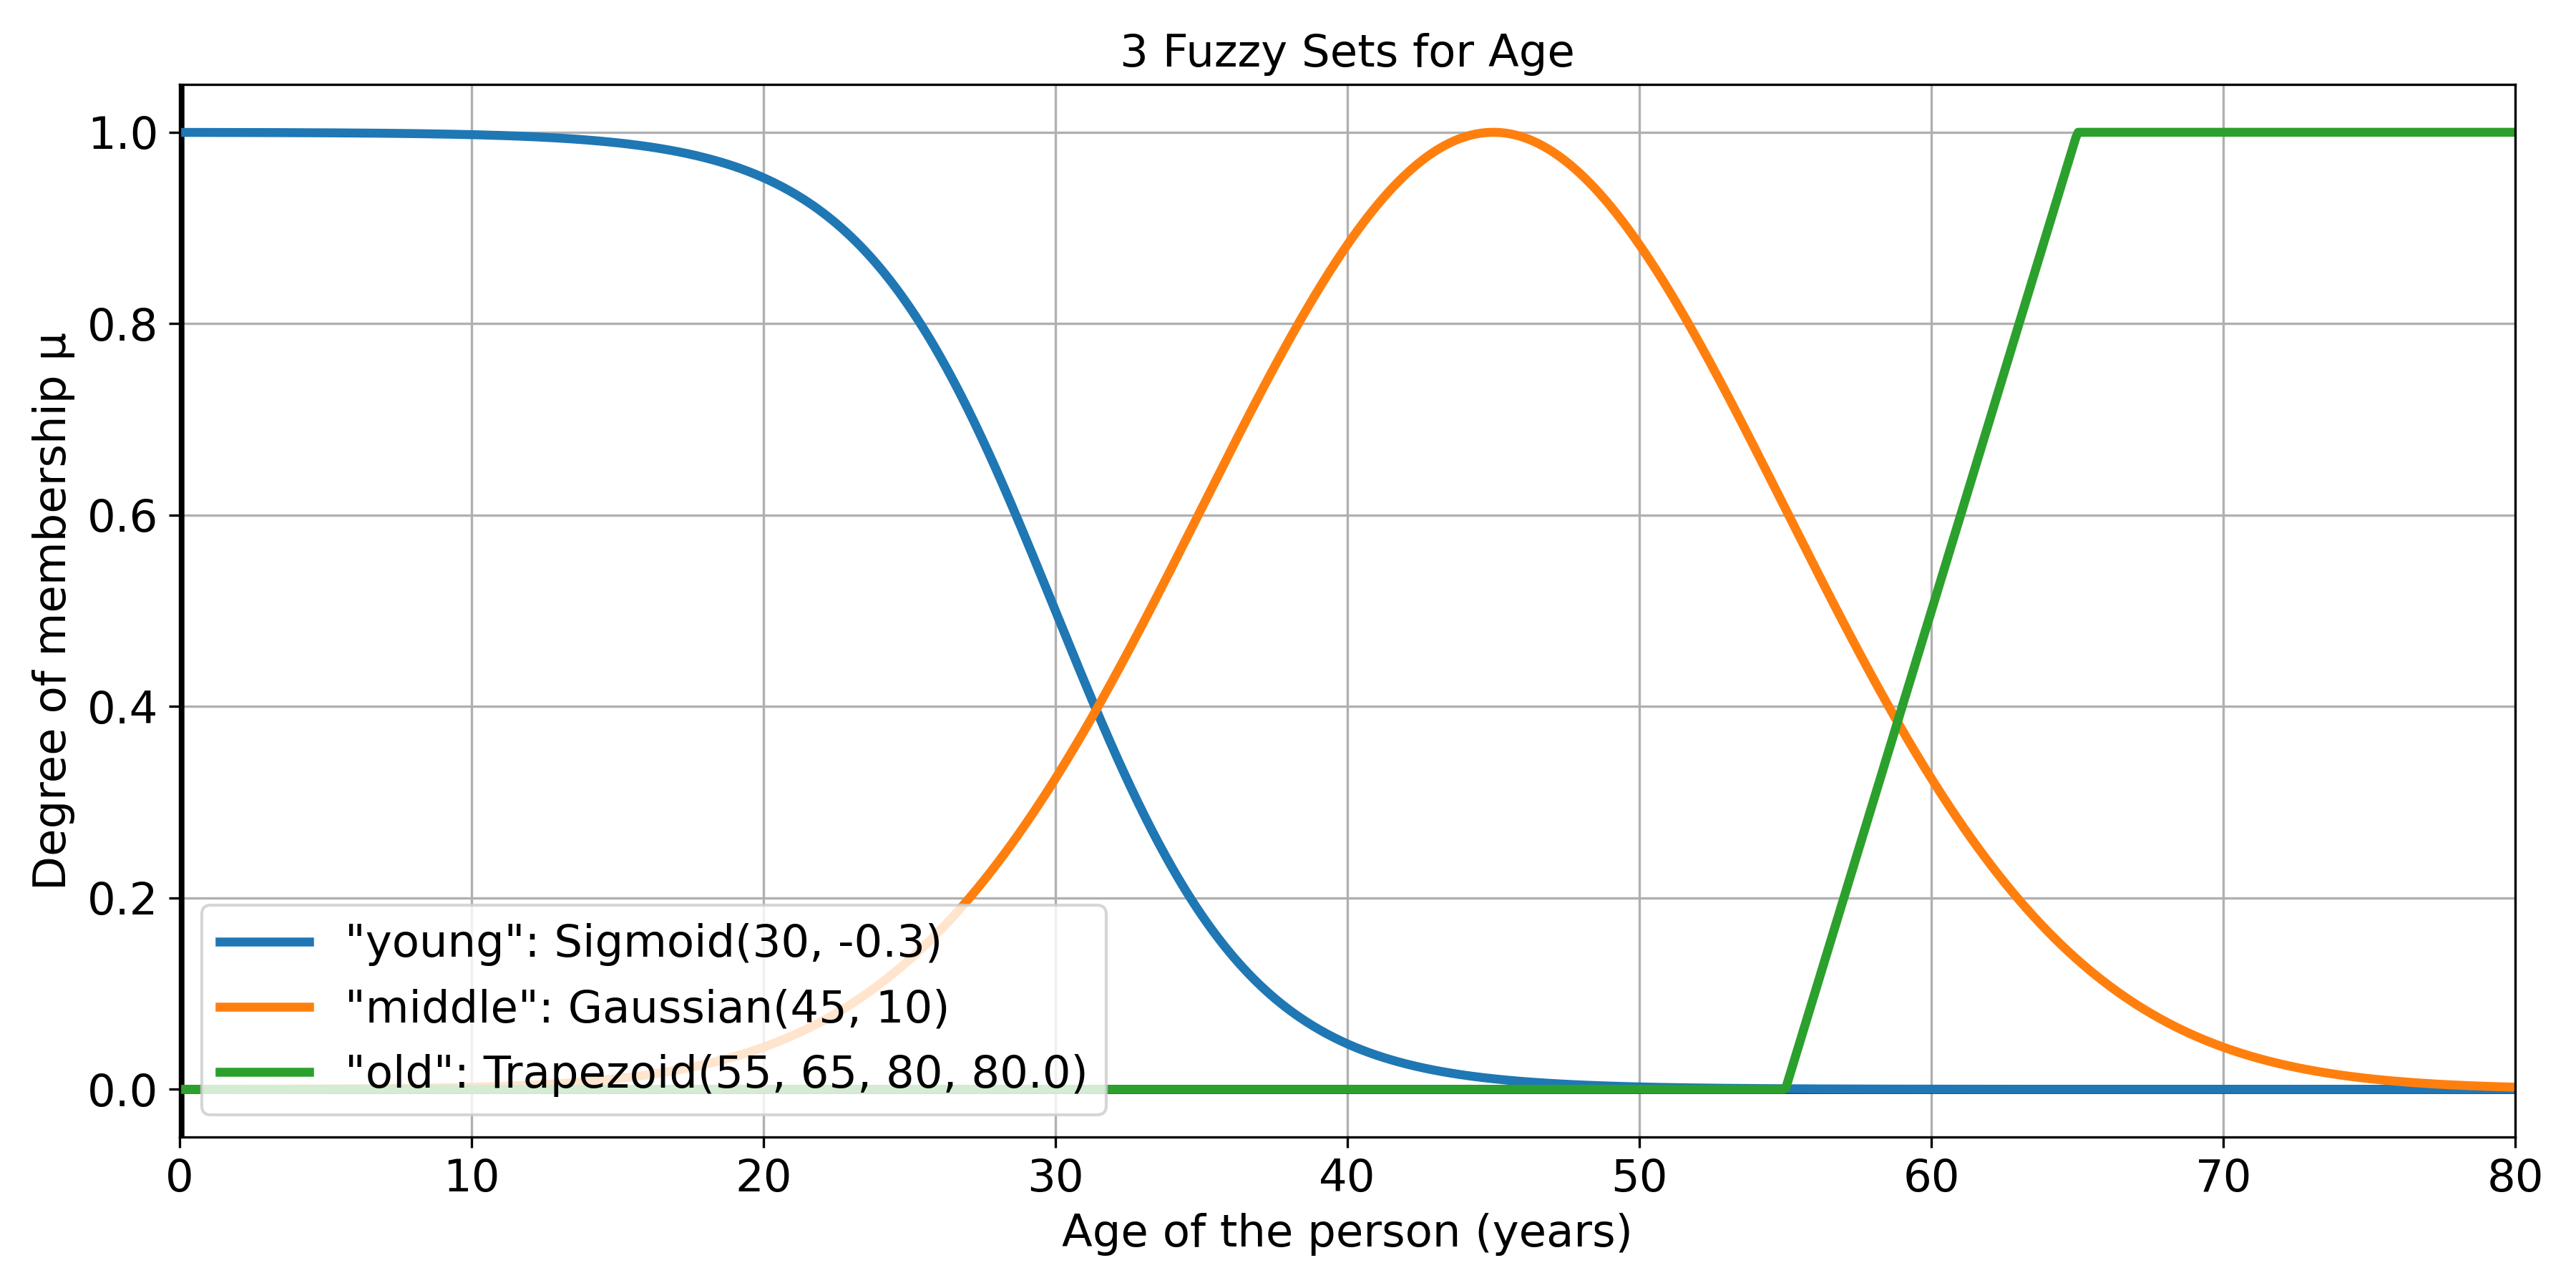
\includegraphics[width=0.8\textwidth,trim={0 0.1cm 0 1.2cm},clip]{figures/age-fuzzy-sets.png}
	\end{center}
\end{frame}

\begin{frame}
	\frametitle{Linguistic Variables}
	\begin{itemize}
		\item Linguistic Variables can take linguistic terms (fuzzy sets)
		      \begin{itemize}
			      \item E.g. \textit{age} can take \textit{young}, \textit{middle-aged} or \textit{old}
		      \end{itemize}
		\item Instead of using crisp values (35 years), we use a combination of linguistic terms to describe the age (Fuzzyification):
		      \[ \text{ 35 years} \implies  \begin{cases}
				      \text{20\% young}       \\
				      \text{60\% middle-aged} \\
				      \text{0\% old}
			      \end{cases}
		      \]
		\item This allows for non-numerical reasoning:
		      \begin{itemize}
			      \item E.g. \textbf{IF} age is \textit{young} \textbf{THEN} fitness is \textit{high}
			      \item Use abstract concepts instead of crisp values
		      \end{itemize}
		\item Each linguistic term represents a certain \textit{collection} of values with varying degrees of membership
	\end{itemize}
\end{frame}

\begin{frame}
	\frametitle{Fuzzy Logic Operators}
	\begin{itemize}
		\item Fuzzy Logic Operators are used to modify/combine fuzzy sets
		\item Extension of boolean logic operators to real numbers
		      \begin{itemize}
			      \item $\wedge : \{false, true\} \times \{false, true\} \rightarrow \{false, true\}$
			      \item $\textbf{AND} : [0,1] \times [0,1] \rightarrow [0,1]$
		      \end{itemize}
		\item Fuzzy operators defined via extension of set
		      \begin{itemize}
			      \item Need to maintain the classical semantics
			      \item Boolean logic is a special case of fuzzy logic
		      \end{itemize}

		\item Typically, Fuzzy Logic Operators are defined as:
		      \begin{itemize}
			      \item \textbf{AND:} Corresponds to the intersection of fuzzy sets
			            \[ \mu_{\tilde{A} \cap \tilde{B}}(x) = \min(\mu_{\tilde{A}}(x), \mu_{\tilde{B}}(x)) \]
			      \item \textbf{OR:} Corresponds to the union of fuzzy sets
			            \[ \mu_{\tilde{A} \cup \tilde{B}}(x) = \max(\mu_{\tilde{A}}(x), \mu_{\tilde{B}}(x)) \]
			      \item \textbf{NOT:} Corresponds to the complement of a fuzzy set
			            \[ \mu_{\neg \tilde{A}}(x) = 1 - \mu_{\tilde{A}}(x) \]

		      \end{itemize}
	\end{itemize}
\end{frame}

\begin{frame}
	\vspace{0cm}
	\begin{figure}
		\centering
		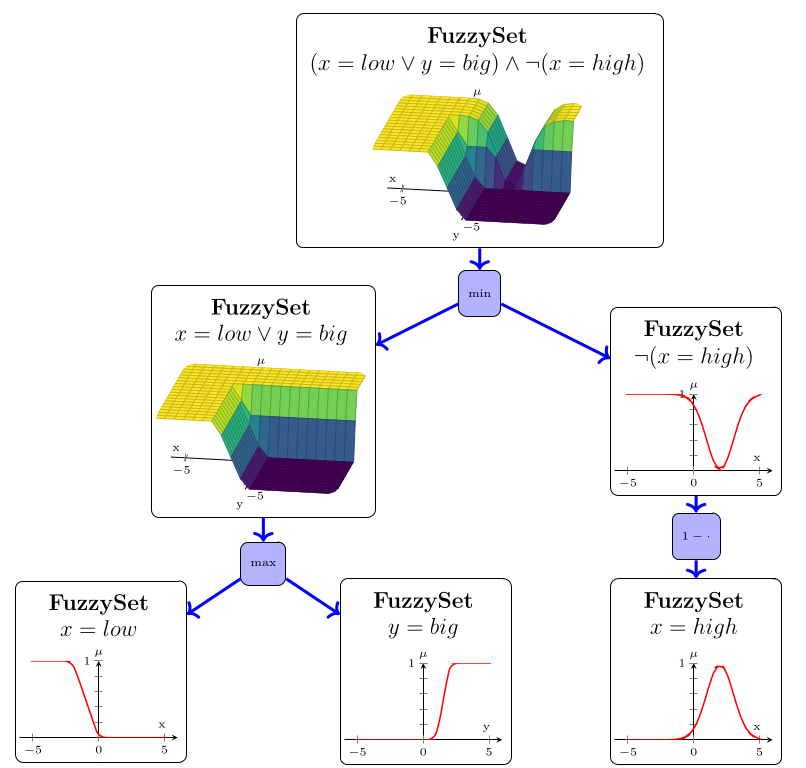
\includegraphics[height=0.62\paperwidth]{figures/RecursiveFuzzyTree.png}
	\end{figure}
\end{frame}

\begin{frame}
	\frametitle{Fuzzy Rules}
	\begin{itemize}
		\item Each rule is of the form: $\textbf{IF} \; {antecedent} \; \textbf{THEN} \; {consequent}$
		      \begin{itemize}
			      \item Both \textit{antecedent} and \textit{consequent} are fuzzy sets
			      \item E.g. $\textbf{IF} \; \text{age} \; \text{is} \; \textit{young} \; \textbf{THEN} \; \text{fitness} \; \text{is} \; \textit{high}$
		      \end{itemize}
		\item Rules are evaluated as logical implications
		      \begin{itemize}
			      \item $\textbf{IF} \; \tilde{A} \; \textbf{THEN} \; \tilde{B} \quad \iff \quad \tilde{A} \;  \textbf{IMPLIES} \;  \tilde{B}$
			      \item Special form of (fuzzy) implication: Mamdani Implication
			            \begin{itemize}
				            \item $\tilde{R} = \textbf{IF} \; \tilde{A} \; \textbf{THEN} \; \tilde{B}$
				            \item $\mu_{\tilde{R}}(x) = \min(\mu_{\tilde{A}}(x), \mu_{\tilde{B}}(x))$
			            \end{itemize}
			      \item \textit{Effect} of the rule is limited by the \textit{strength} of the antecedent
		      \end{itemize}
		\item Multiple rules can act on the same linguistic variable
		      \begin{itemize}
			      \item The total \textit{effect} on the output is the aggregation/union of all individual fuzzy sets
			      \item Each rule \textit{effect} is considered proportional to the \textit{strength} of its antecedent
		      \end{itemize}
	\end{itemize}
\end{frame}

\begin{frame}
	\frametitle{Defuzzification}
	\begin{itemize}
		\item Process of converting arbitrary fuzzy sets to a crisp value
		      \begin{itemize}
			      \item Special case: Fuzzy sets corresponding to a fuzzification
			            \[  \begin{cases}
					            \text{20\% young}       \\
					            \text{60\% middle-aged} \\
					            \text{0\% old}
				            \end{cases} \implies \text{35 years}
			            \]
		      \end{itemize}
		\item Multiple methods for defuzzification:
		      \begin{itemize}
			      \item \textbf{Center of Gravity:} Considers all values based on their membership. Finds weighted average of all possible values
			      \item \textbf{Mean of Maxima:} Considers only the most likely values (with highest membership). Finds the mean of all maxima
		      \end{itemize}
		\item Core idea: Represent aspects of the fuzzy set with a crisp value
		      \begin{itemize}
			      \item E.g. Weighted average of all possible values (Centroid)
			      \item E.g. Most likely value (Mean of Maxima)
		      \end{itemize}
	\end{itemize}

\end{frame}



\begin{frame}
	\vspace{-0.8cm}
	\begin{figure}
		\centering
		\caption{\tiny{Source: \href{https://de.mathworks.com/help/fuzzy/fuzzy-inference-process.html}{MathWorks - Fuzzy Inference Process}}}
		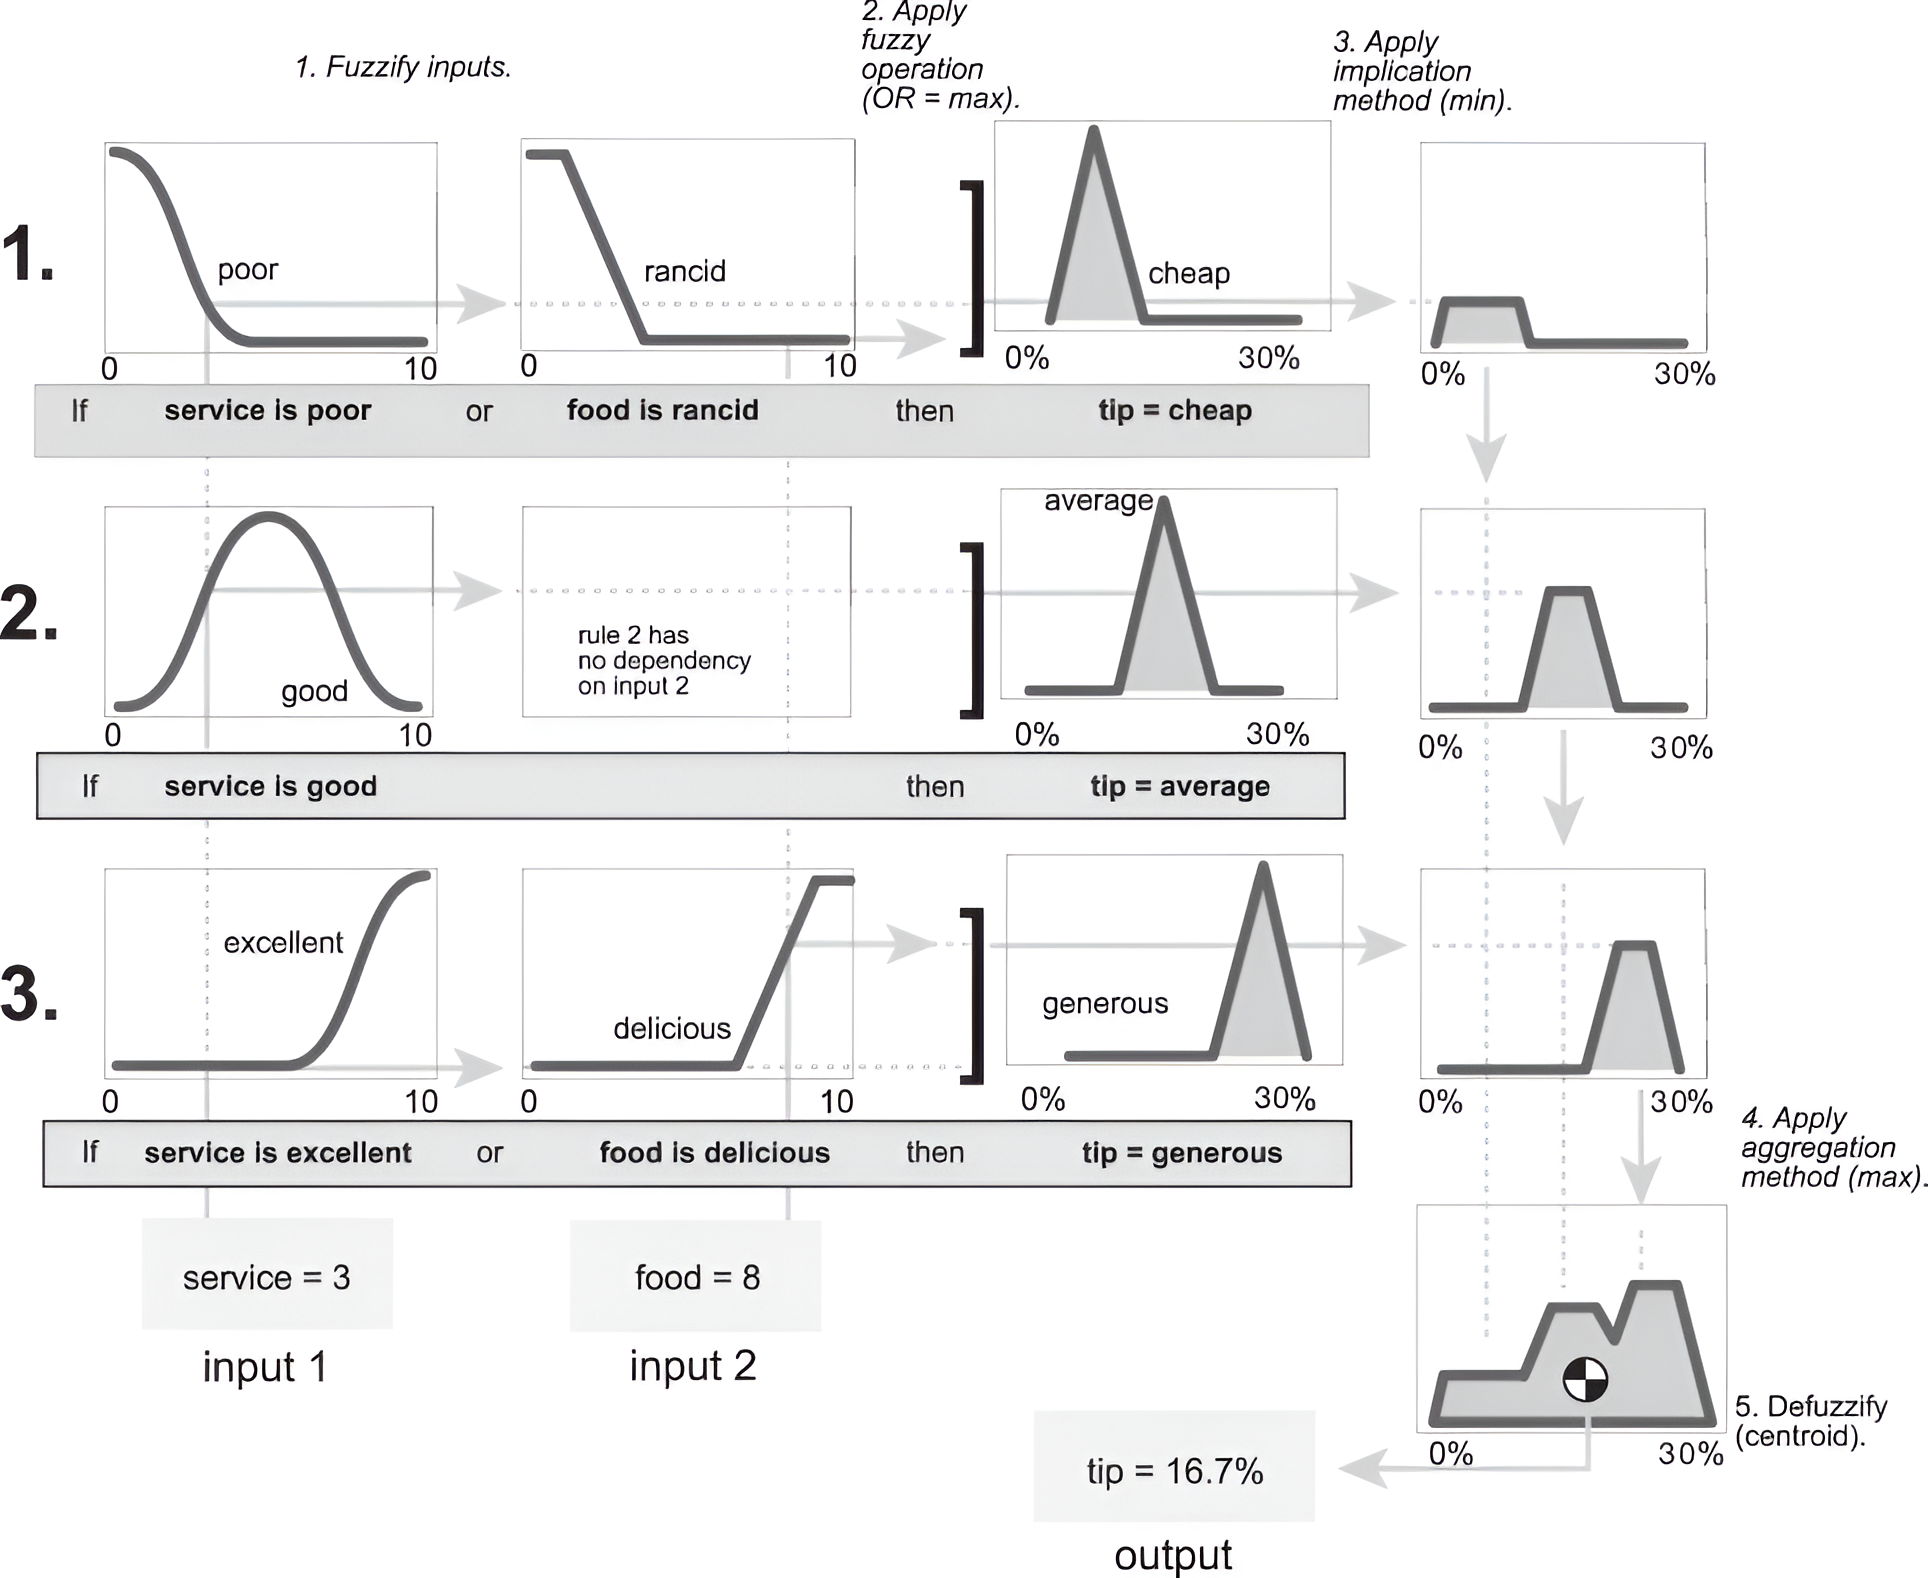
\includegraphics[width=0.8\paperwidth]{figures/FullInferenceProcess.png}
	\end{figure}
	\label{fig:fuzzy_inference_full}

\end{frame}


\section{Fuzzy Tuning Strategy for AutoPas}
\begin{frame}
	\frametitle{Fuzzy Tuning Strategy}

	\begin{itemize}
		\item Main Idea: Use Fuzzy Logic to tune AutoPas
		\item Make use of LiveInfoData\footnote{Simulation state: \texttt{avgParticles/Cell, homogeneity, threadCount \dots }} to perform tuning
		\item Advantages:
		      \begin{itemize}
			      \item Expert knowledge can provide powerful tuning
			      \item Potentially more robust against noise
			      \item May require fewer rules than rule-based tuning
			      \item Easy to interpret and understand
		      \end{itemize}
		\item Challenges and Questions:
		      \begin{itemize}
			      \item What are the output variables? How to predict Configurations?
			      \item How to interpret the result? (Fuzzy System : $f :\mathbb{R}^n \rightarrow \mathbb{R}$ )
			      \item How to create the fuzzy rules and linguistic terms?
			            \begin{itemize}
				            \item Expert knowledge?
				            \item Machine Learning?
			            \end{itemize}
		      \end{itemize}
	\end{itemize}
\end{frame}

\section{Approaches for Fuzzy Tuning in AutoPas}
\subsection{Component Tuning}
\begin{frame}
	\frametitle{Approach 1: Component Tuning}
	\begin{itemize}
		\item Predict good values/patterns for each tunable parameter separately
		\item A Fuzzy System for each tunable parameter
		      \begin{itemize}
			      \item Output Variable: Class values of the parameter
			      \item Idea: Map numerical output of the Fuzzy System to the \textit{closest} class value {\footnotesize \cite{Mohammed2022}}
		      \end{itemize}
		\item Combine all results to find resulting configuration(s)
	\end{itemize}

	\begin{figure}
		\centering
		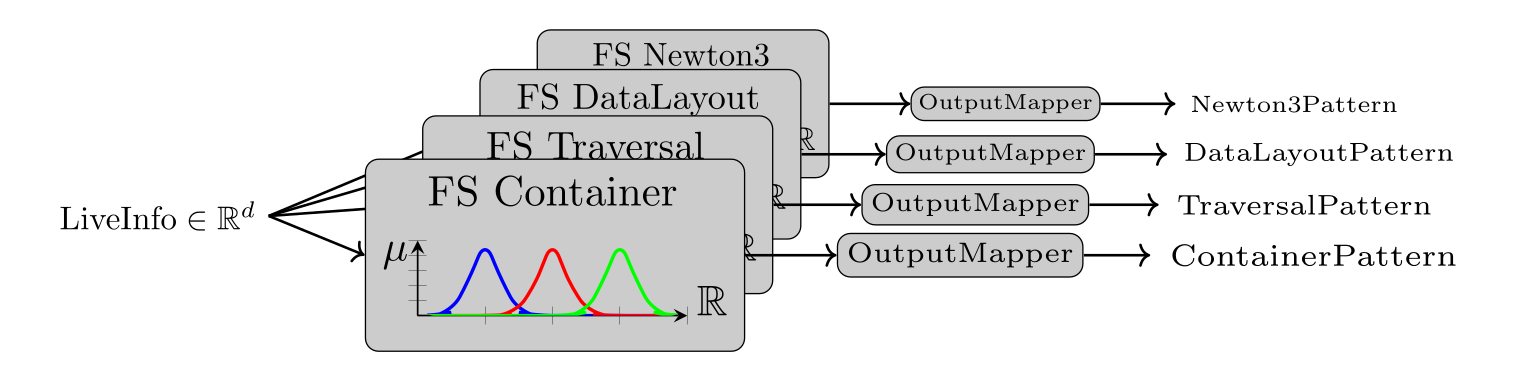
\includegraphics[width=1\textwidth]{figures/component-approach.png}
	\end{figure}

\end{frame}

\begin{frame}
	\frametitle{Approach 1: Component Tuning (Example)}
	\begin{itemize}
		\item Style: {\small \textbf{IF} avgParticlesPerCell is \textit{low} \textbf{AND} threadCount is \textit{low}\\ \qquad  \qquad \quad \textbf{THEN} traversal is \textit{vcl\_c06}}
		\item \textbf{Benefits:}
		      \begin{itemize}
			      \item Few fuzzy systems
			      \item Few and natural rules
		      \end{itemize}
		\item \textbf{Drawbacks:}
		      \begin{itemize}
			      \item Unused power of fuzzy logic (MoM defuzzification)
			      \item Independence assumption
		      \end{itemize}


	\end{itemize}

	\begin{figure}
		\centering
		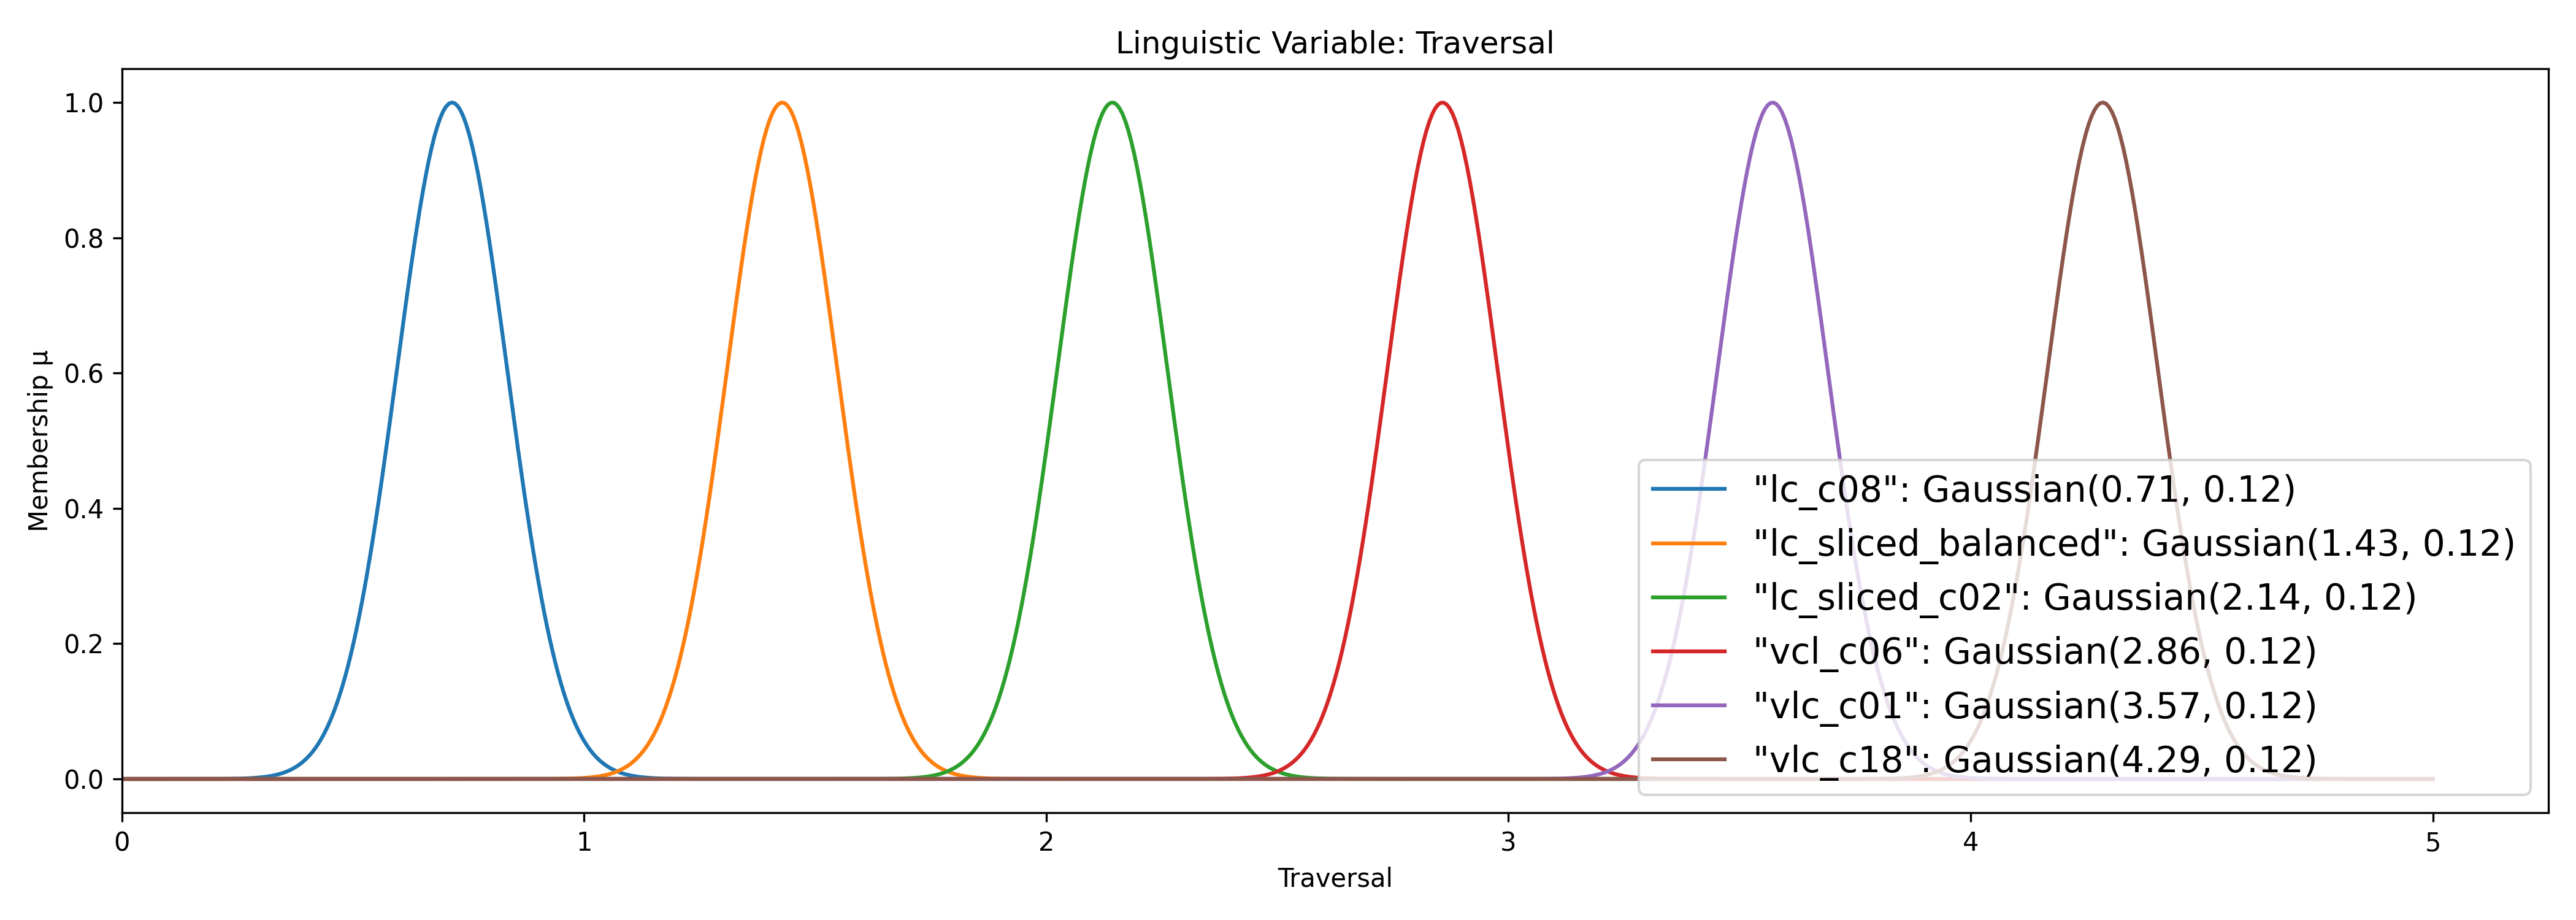
\includegraphics[width=0.9\textwidth,trim={0 0 0 1cm},clip]
		{figures/component-linguistic-variable.png}
	\end{figure}

\end{frame}



\subsection{Suitability Tuning}

\begin{frame}
	\frametitle{Approach 2: Suitability Tuning}
	\begin{itemize}
		\item Predict the suitability of \textit{each} configuration
		\item A Fuzzy System for each possible configuration
		      \begin{itemize}
			      \item Output Variable: Suitability classes of the configuration
			      \item Directly use numerical output as suitability value
		      \end{itemize}
		\item Configuration with high suitabilities are chosen
	\end{itemize}

	\begin{figure}
		\centering
		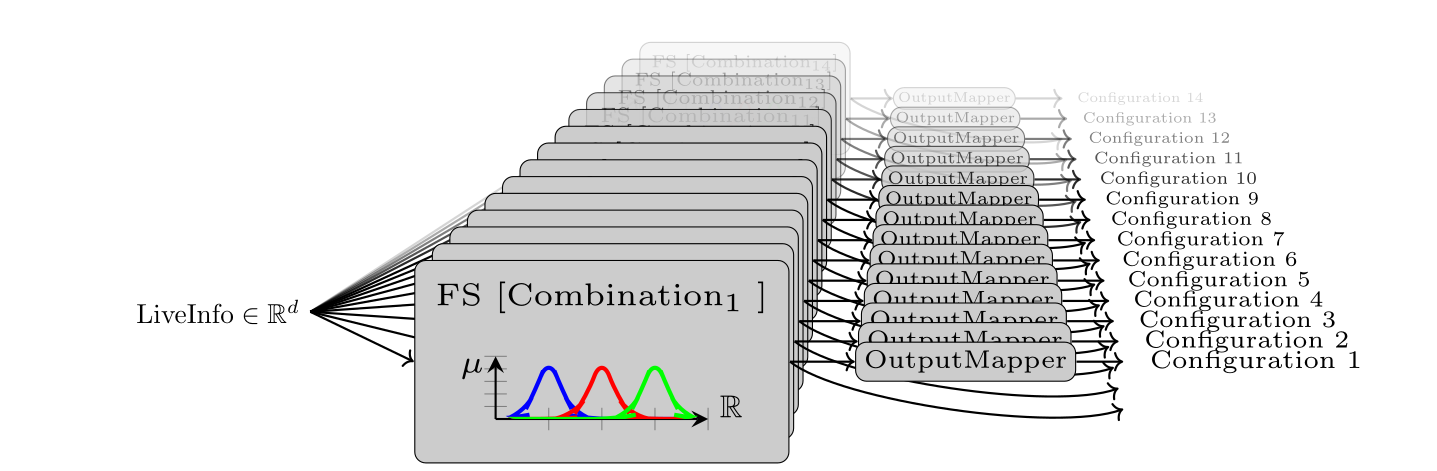
\includegraphics[width=1\textwidth]{figures/suitability-approach.png}
	\end{figure}
\end{frame}


\begin{frame}
	\frametitle{Approach 2: Suitability Tuning (Example)}
	\begin{itemize}
		\item Style: {\small
		      \textbf{IF} threadCount is \textit{high} \textbf{AND} avgParticlesPerCell is \textit{low}\\ \qquad \qquad \quad \textbf{THEN} suitability\_LinkedCells\_AoS\_lc\_c18\_disabled is \textit{bad}}

		\item \textbf{Benefits:}
		      \begin{itemize}
			      \item Utilizes the full power of fuzzy logic (CoG defuzzification)
			      \item Dependencies and incompatibilities can be modeled
		      \end{itemize}
		\item \textbf{Drawbacks:}
		      \begin{itemize}
			      \item Huge number of fuzzy systems
			      \item Impossible to maintain by hand
		      \end{itemize}
	\end{itemize}

	\begin{figure}
		\centering
		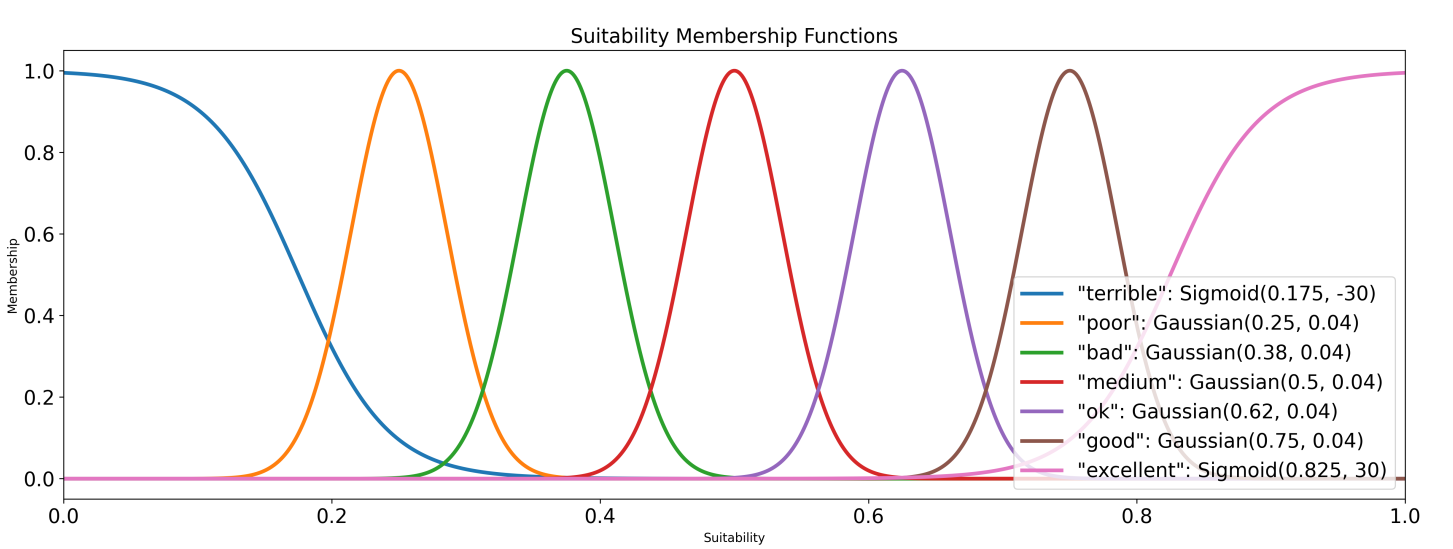
\includegraphics[width=0.82\textwidth,trim={0 0 0 1.8cm},clip]{figures/suitability-linguistic-variable.png}
	\end{figure}

\end{frame}


\section{Data-Driven Rule Extraction Process}
\begin{frame}
	\frametitle{Data-Driven Rule Extraction}
	\begin{itemize}
		\item Creating the Fuzy Rules and Linguistic Terms manually is difficult
		      \begin{itemize}
			      \item Expert Knowledge is required
			      \item Formalization of knowledge is difficult
			      \item Potentially many rules required
		      \end{itemize}
		\item Use Machine Learning to extract rules from data
		      \begin{itemize}
			      \item Decision Tree $\rightarrow$ Fuzzy Decision Tree $\rightarrow$ Fuzzy Rules {\footnotesize \cite{CROCKETT20062809}}
			      \item Does not require expert knowledge
		      \end{itemize}
		\item Human experts can still validate the rules
	\end{itemize}
\end{frame}

\begin{frame}
	\frametitle{Decision Trees}

	\begin{itemize}
		\item \textbf{Idea}: Split data with axis-aligned splits to best separate classes
		\item Corresponds to nested \textit{if-then-else} rules
		\item Easy to understand and interpret
		\item TFinal tree contains the entire expert knowledge
		\item Can be trained automatically, given enough data
		      \begin{itemize}
			      \item No expert knowledge required!
		      \end{itemize}
	\end{itemize}

	\begin{figure}
		\centering
		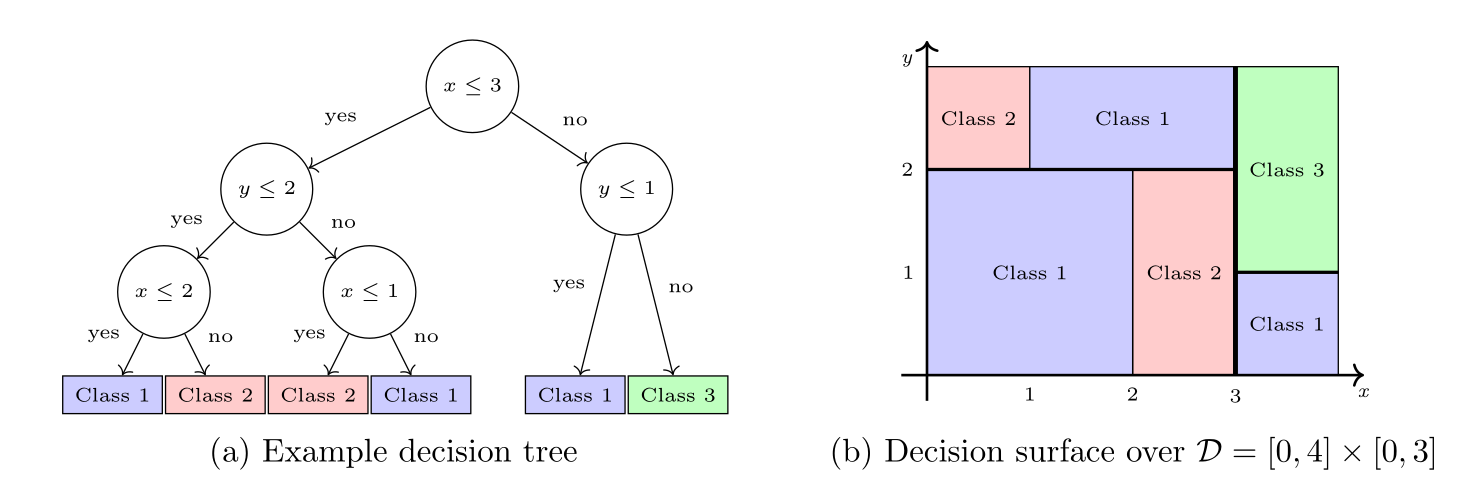
\includegraphics[width=1\textwidth]{figures/decision-tree.png}
	\end{figure}

\end{frame}

\begin{frame}
	\frametitle{Decision Trees $\rightarrow$ Fuzzy Decision Trees}

	\begin{itemize}
		\item Fuzzy Decision Trees
		      \begin{itemize}
			      \item Each decision is a linguistic term
			      \item E.g. Traverse left if temperature is \textit{cold}
		      \end{itemize}
		\item Conversion: Each (crisp) split is turned into two fuzzy sets
		      \begin{itemize}
			      \item Fuzzy sets should maintain the semantics of the split
			      \item Provides robustness against noise
		      \end{itemize}
		\item Leaf nodes are represented with Linguistic terms
	\end{itemize}
	\begin{figure}
		\centering
		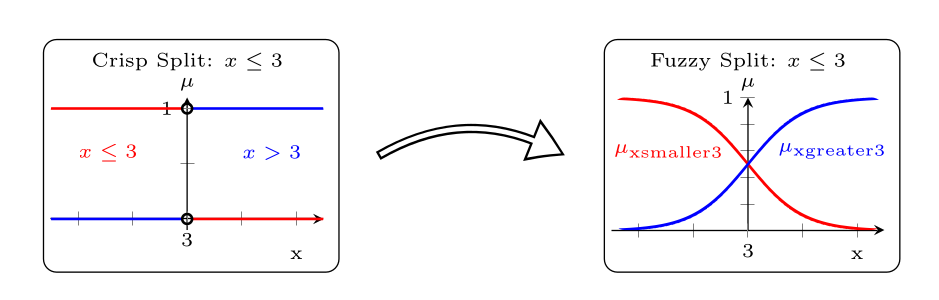
\includegraphics[width=8cm]{figures/leaf-conversion.png}
	\end{figure}

\end{frame}

\begin{frame}

	\begin{figure}
		\centering
		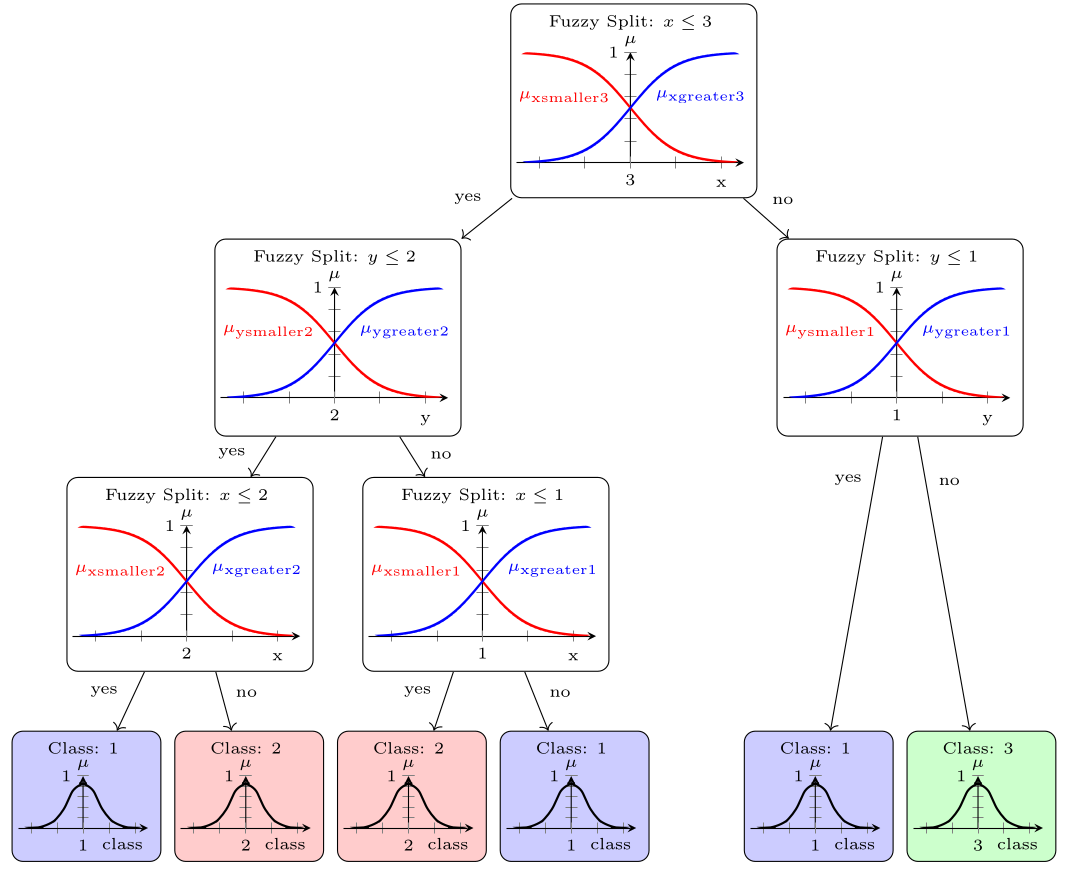
\includegraphics[width=0.9\textwidth]{figures/fuzzy-decision-tree.png}
	\end{figure}

\end{frame}

\begin{frame}

	\frametitle{Fuzzy Decision Trees $\rightarrow$ Fuzzy Rules}

	\begin{itemize}
		\item Depth-First traversal of the Fuzzy Decision Tree
		      \begin{itemize}
			      \item Each node corresponds to a condition ofthe antecedent
			      \item Leaf node corresponds to the consequent
		      \end{itemize}
		\item One rule per path from root to leaf
		\item Corresponds to \textit{unnesting} the decision tree
	\end{itemize}

	\begin{figure}
		\centering
		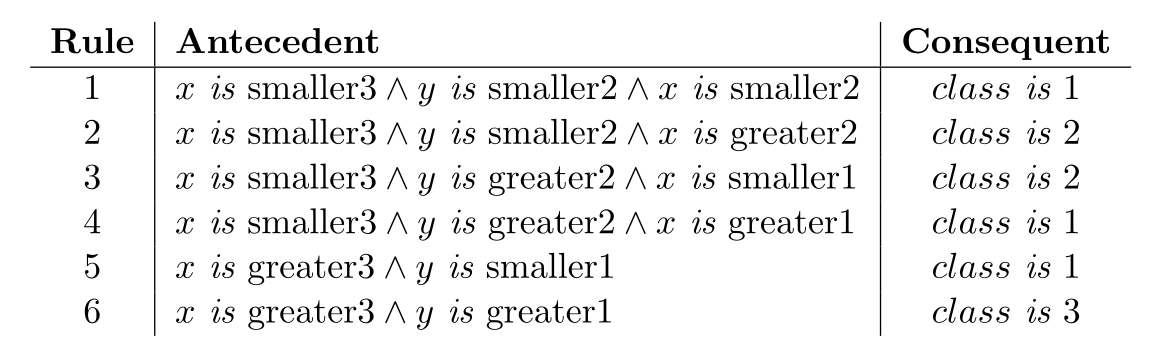
\includegraphics[width=0.9\textwidth]{figures/extracted-rules.png}
	\end{figure}

\end{frame}

\begin{frame}

	\frametitle{Fuzzy Decision Surfaces - CoG vs. MoM}

	\begin{itemize}
		\item CoG: Interpolation effect + errors, smooth boundaries
		\item MoM: Hard boundaries, similar to Decision Trees
	\end{itemize}

	\begin{figure}
		\centering
		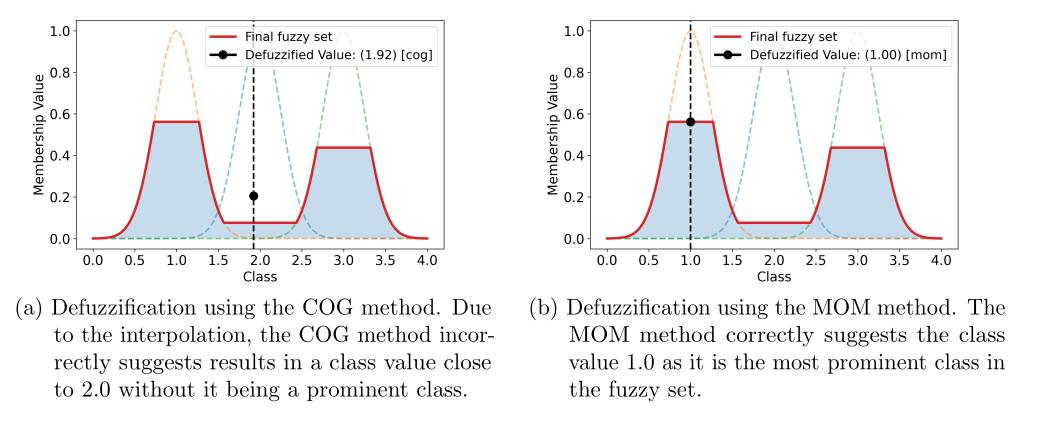
\includegraphics[width=0.87\textwidth, trim={0 4.8cm 0 0cm},clip]{figures/cog-vs-mom.png}

		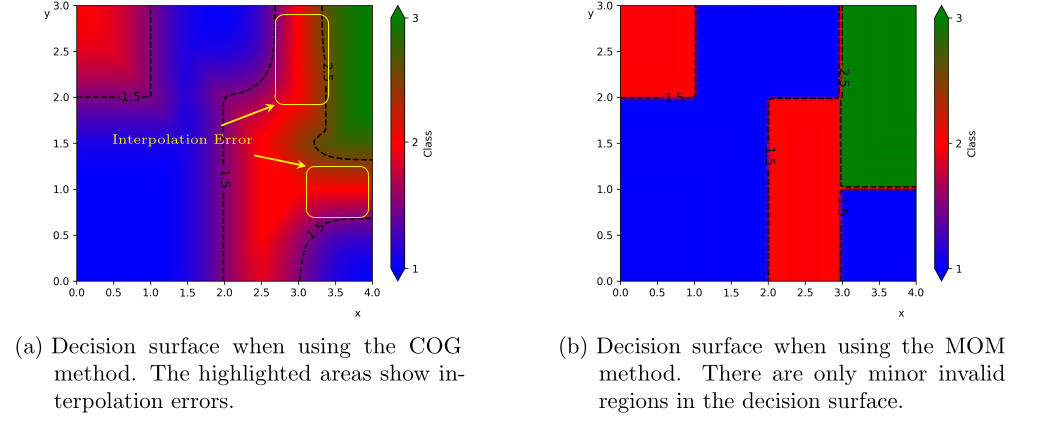
\includegraphics[width=0.88\textwidth, trim={0 3.8cm 0 0cm},clip]{figures/decision-surfaces.png}
	\end{figure}


\end{frame}


\section{Fuzzy Rule Extraction for \texttt{md\_flexible}}
\begin{frame}
	\frametitle{Fuzzy Rule Extraction for \texttt{md\_flexible}}

	\begin{itemize}
		\item Collect huge dataset of \texttt{md\_flexible} simulations
		\item LiveInfoData: {\small \texttt{maxDensity, homogeneity, threadCount, \dots} }
		\item TuningData: {\small \texttt{Container, Traversal, Newton3, \dots, Time} }
		\item Introduce notion of \textit{relative speed} for each configuration
		      \begin{itemize}
			      \item $t_{best}^{(i)}$: Best configuration time in tuning phase $i$
			      \item $t_{config}^{(i)}$: Time of configuration in tuning phase $i$
			            \[ \text{relative speed}_{config}^{(i)} = \frac{\text{t}_{best}^{(i)}}{\text{t}_{\text{config}}^{(i)}} \]
			      \item Allows for fair comparison between different tuning phases
		      \end{itemize}
	\end{itemize}

\end{frame}

\begin{frame}
	\frametitle{Resulting Dataset}

	\begin{itemize}
		\item Performance of configurations in different environments
		\item Can be used to extract rules for both approaches
		\item Goal: Find configurations with high relative speed
	\end{itemize}

	\begin{figure}
		\centering
		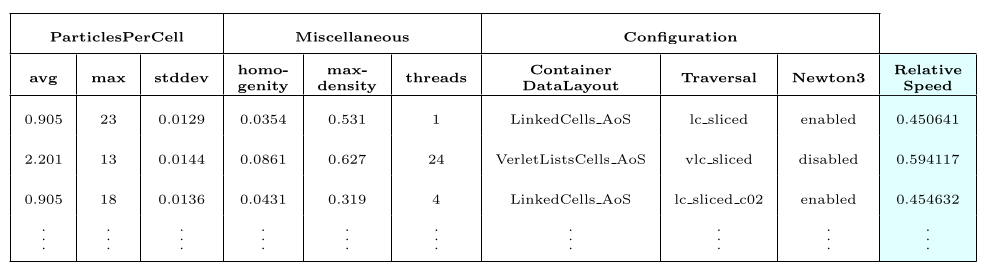
\includegraphics[width=1\textwidth]{figures/relative-speed-table.png}
	\end{figure}

\end{frame}

\begin{frame}
	\frametitle{Generate Rules: Approach 1}

	\begin{itemize}
		\item Naively remove bad configurations (relative speed $<70\%$)
		\item Group remaining dataset by tuning-phase (same live-info)
		\item Aggregate present (\textit{good}) values for each parameter
		\item Apply Rule Extraction algorithm to each parameter
	\end{itemize}

	\begin{figure}
		\centering
		\vspace{-0.1cm}
		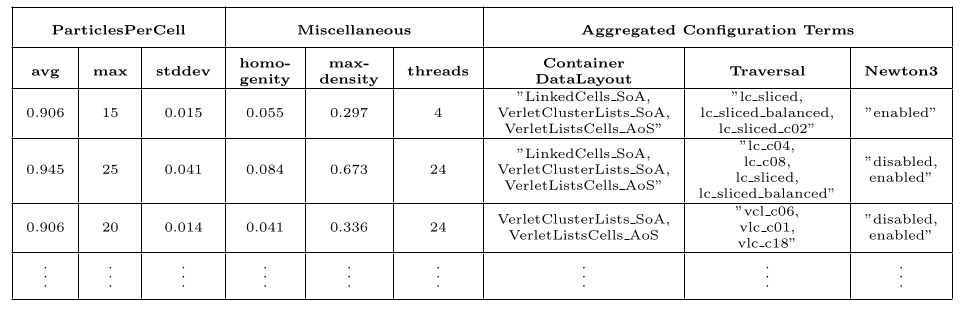
\includegraphics[width=0.95\textwidth, trim={0 3.8cm 0 0},clip]{figures/aggregated-data-component.png}
		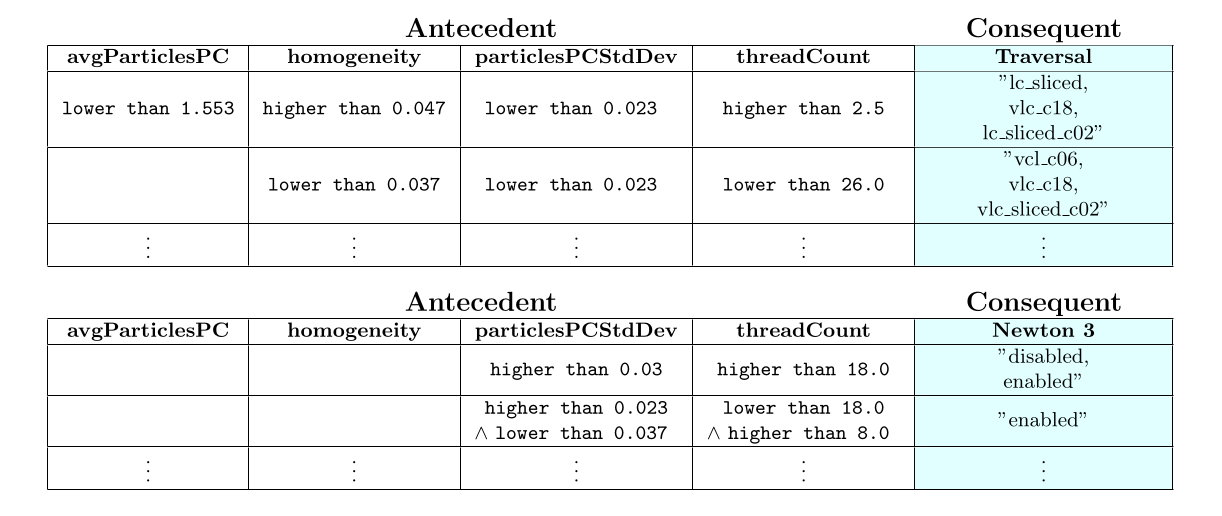
\includegraphics[width=1\textwidth, trim={0 8cm 0 0},clip]{figures/final-rules-component.png}
	\end{figure}
\end{frame}

\begin{frame}
	\frametitle{Generate Rules: Approach 2}

	\begin{itemize}
		\item Assign suitability-classes to each entry in the dataset
		\item Classes represent ranges of relative speed
		\item Apply Rule Extraction algorithm for the suitability class
	\end{itemize}

	\begin{figure}
		\centering
		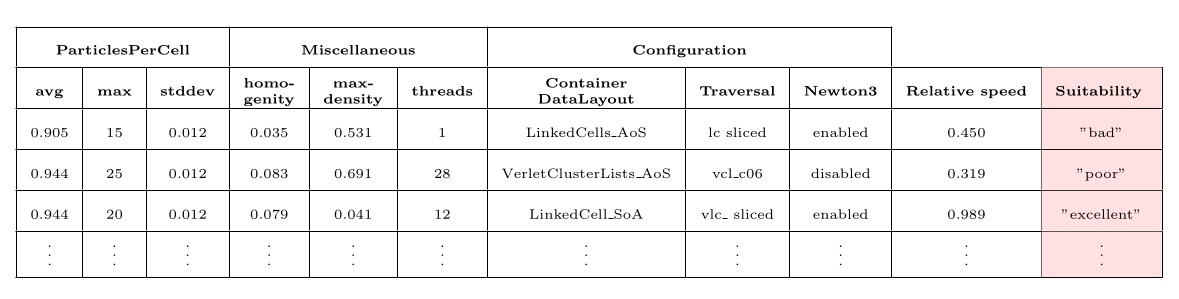
\includegraphics[width=1\textwidth, trim={0 2.25cm 0 0},clip]{figures/aggregated-data-suitability.png}
		\vspace{1.5cm}
		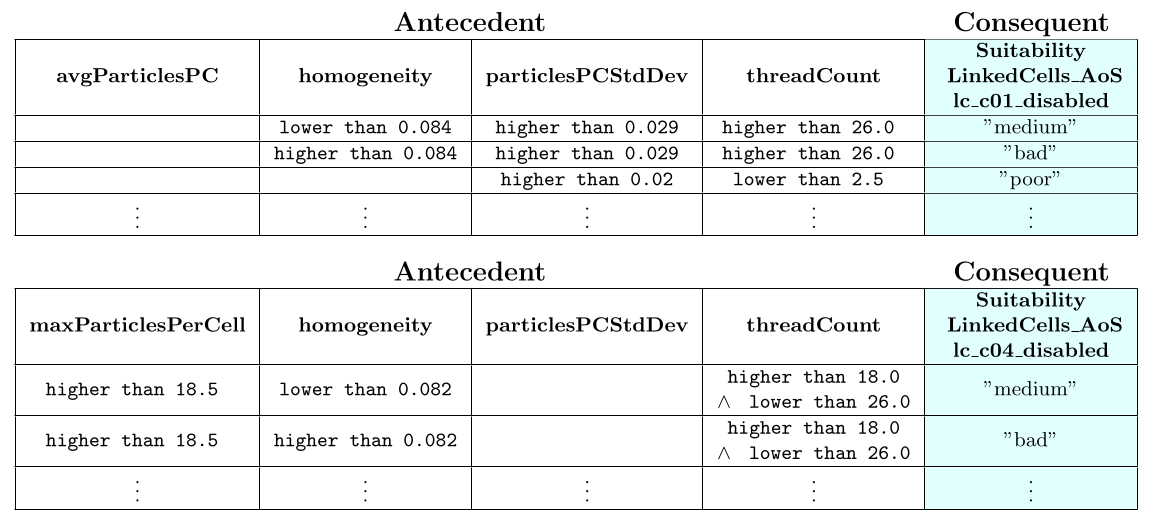
\includegraphics[width=1\textwidth, trim={0 9cm 0 0.1cm},clip]{figures/final-rules-suitability.png}
	\end{figure}
\end{frame}

\section{Benchmarks}
\subsection{Exploding Liquid}
\begin{frame}
	\frametitle{Benchmark 1: Exploding Liquid}
	\begin{itemize}
		\item Exploding Liquid Benchmark (Included in Dataset)
		      \begin{itemize}
			      \item Both fuzzy approaches look promising
			      \item Very short tuning phases (not much noise)
			      \item Selected configurations perform well (tiny spikes)
			      \item Winning configurations are (mostly) equivalent
		      \end{itemize}
	\end{itemize}

	\begin{figure}
		\centering
		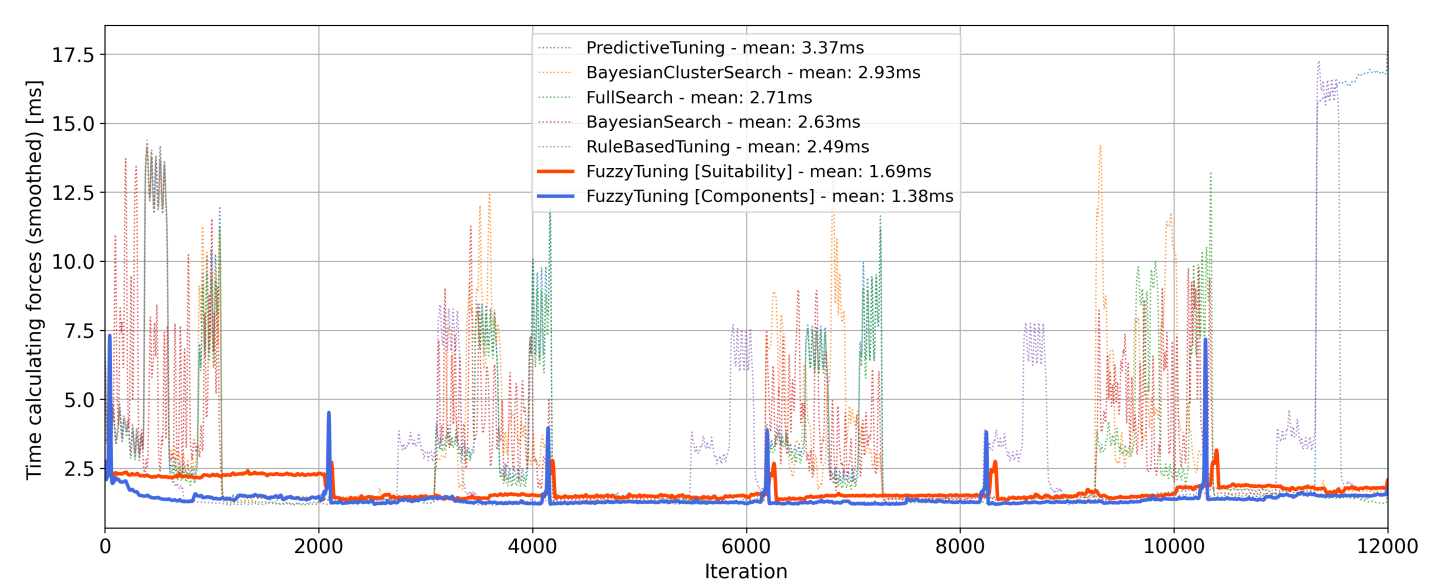
\includegraphics[width=1\textwidth]{figures/exploding-liquid-timings.png}
	\end{figure}
\end{frame}

\begin{frame}
	\frametitle{Total Time: Exploding Liquid}
	\begin{itemize}
		\item Fuzzy tuning has lowest total time
		\item Mostly due to the very efficient tuning phases
		      \begin{itemize}
			      \item Few configurations evaluated
			      \item Evaluated configurations are expected to perform well
		      \end{itemize}
		\item Benefits of tuning with tiny overhead
	\end{itemize}

	\begin{figure}
		\centering
		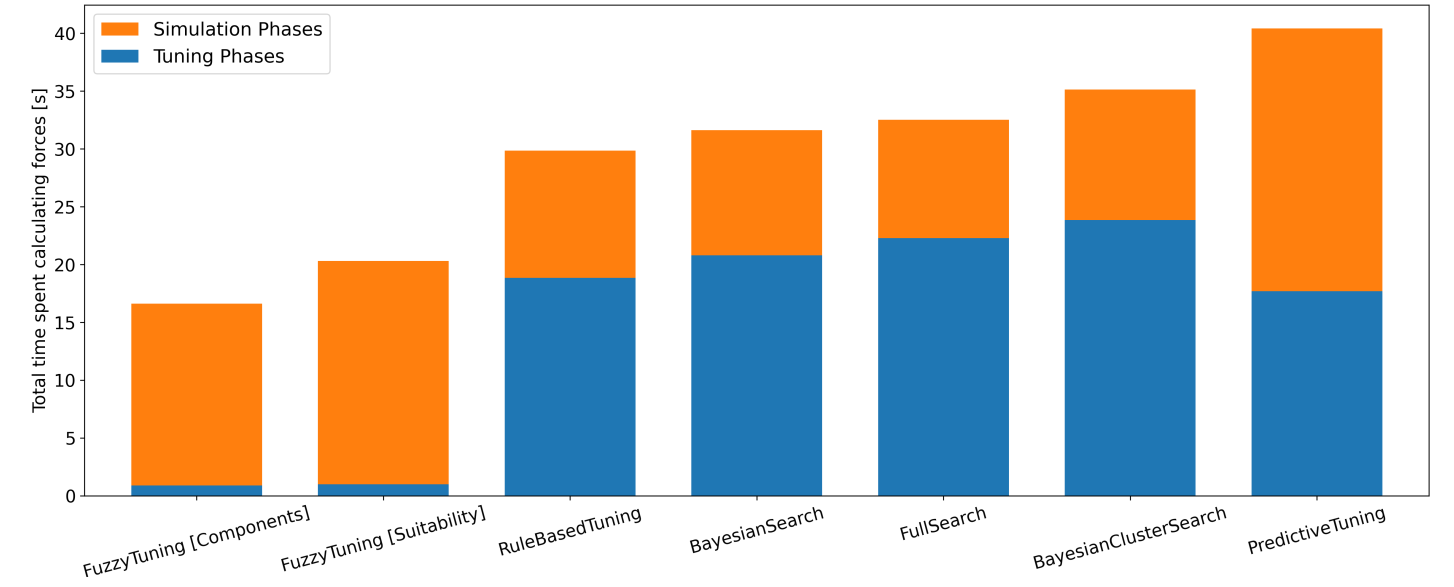
\includegraphics[width=0.95\textwidth]{figures/exploding-liquid-total.png}
	\end{figure}
\end{frame}

\subsection{Spinodal Decomposition}

\begin{frame}
	\frametitle{Benchmark 2: Spinodal Decomposition MPI}

	\begin{itemize}
		\item Spinodal Decomposition MPI (Indirectly included in Dataset)
		      \begin{itemize}
			      \item Fuzzy tuning promising again
			      \item Suitability approach struggles, often misses the best configuration
			      \item However, both approaches have efficient tuning phases
		      \end{itemize}
	\end{itemize}

	\begin{figure}
		\centering
		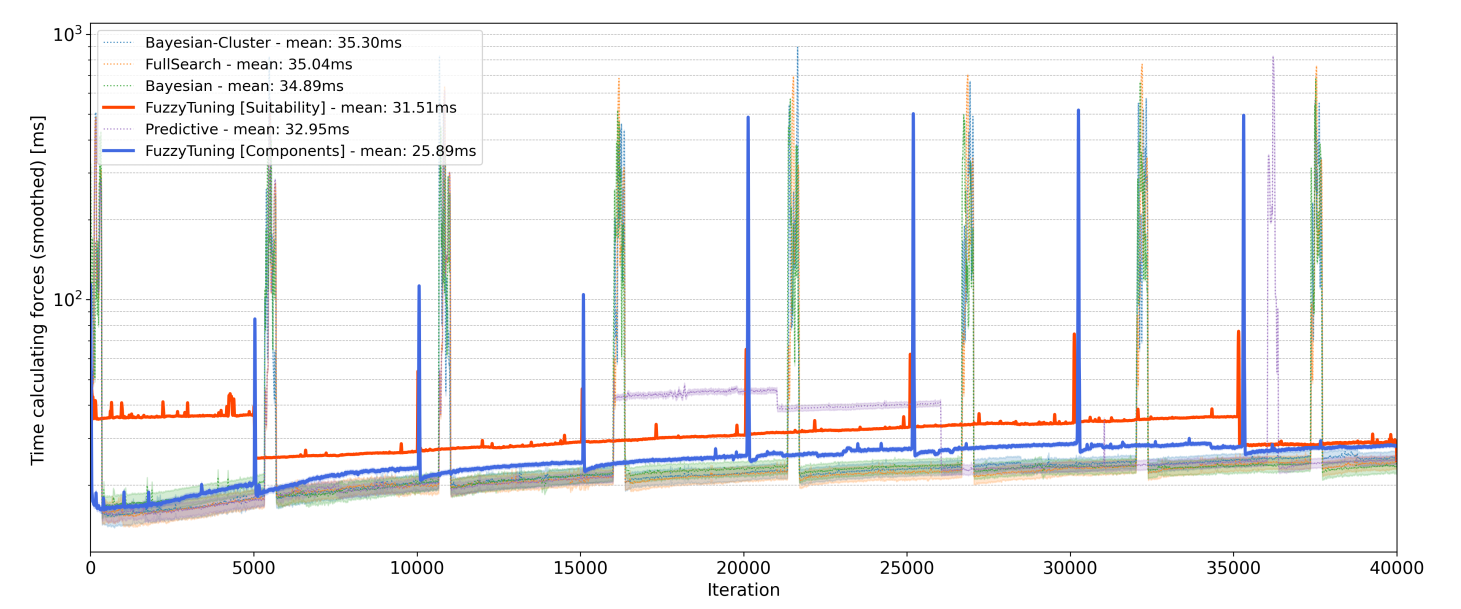
\includegraphics[width=1\textwidth]{figures/spinodal-timings.png}
	\end{figure}
\end{frame}

\begin{frame}
	\frametitle{Comparison and Evaluation: Spinodal Decomposition}

	\begin{itemize}
		\item Component approach performs well
		\item Suitability approach still quite fast
		      \begin{itemize}
			      \item Fast tuning phases compensate for suboptimal configurations!
			      \item Misses caused by to optimisitic suitability threshold

			            \begin{itemize}
				            \item  Too few configurations are slected for evaluation
				            \item \textbf{Solution:} Increase the suitability threshold (Top 10\% $\rightarrow$ Top 30\%)
			            \end{itemize}
		      \end{itemize}

	\end{itemize}

	\begin{figure}
		\centering
		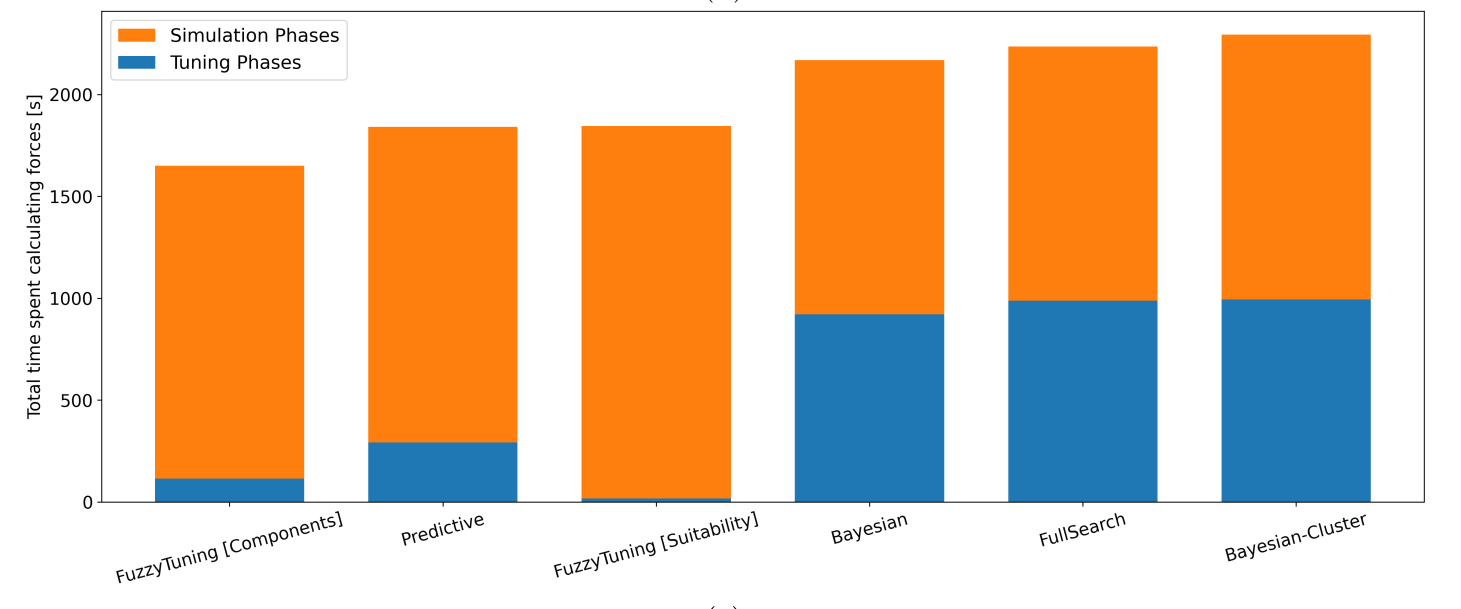
\includegraphics[width=0.92\textwidth]{figures/spinodal-total.png}
	\end{figure}
\end{frame}


\section{Future Work}
\begin{frame}
	\frametitle{Future Work}
	\begin{itemize}
		\item Dynamic Rule Generation
		      \begin{itemize}
			      \item Update the expert knowledge on the fly
			      \item Adapt to new scenarios
			      \item No need for giant datasets
		      \end{itemize}
		\item Improving Tuning Strategies
		      \begin{itemize}
			      \item Implement early stopping mechanism
			      \item Stop evaluating extremely bad configurations early
		      \end{itemize}
		\item Simplification of the Fuzzy System to Decision Trees
		      \begin{itemize}
			      \item Use Decision Trees instead of Fuzzy Systems
			      \item Could potentially perform equally well, while being easier to understand
		      \end{itemize}
	\end{itemize}
\end{frame}


\section{Conclusion}
\begin{frame}
	\frametitle{Conclusion}
	\begin{itemize}
		\item Fuzzy Logic is very promising for tuning AutoPas
		\item Data-Driven Rule Extraction is a powerful tool
		\item However:
		      \begin{itemize}
			      \item Requires a lot of  prior data (current training data is 1.1GB)
			      \item Users cannot be expected to collect this data beforehand
			      \item A more user-friendly approach is needed for broader adoption
		      \end{itemize}
		\item Future work could focus on simplifying/streamlining the rule extraction process
		\item Alternatively: Investigate Early Stopping, to solve the tuning overhead once and for all
	\end{itemize}
\end{frame}

\begin{frame}
	\begin{center}
		\vspace{1cm}
		{\large \textbf{Thank you for your attention!}}

		\vspace{2cm}

		\Huge{Questions?}
	\end{center}
\end{frame}

\thispagestyle{empty}
\begin{frame}[allowframebreaks, noframenumbering]
	\frametitle{References}
	\footnotesize
	\bibliographystyle{apalike}
	\bibliography{literature}
\end{frame}

\end{document}
